\documentclass[runningheads]{llncs}
\usepackage[T1]{fontenc}
\usepackage{graphicx}
\usepackage{booktabs}
\usepackage{array}
\usepackage{microtype}
\usepackage{tikz}

\renewcommand{\topfraction}{.9}\renewcommand{\bottomfraction}{.8}\renewcommand{\textfraction}{.08}\renewcommand{\floatpagefraction}{.75}
\usetikzlibrary{arrows.meta,positioning,fit,backgrounds}
\newcommand{\bfivezerothreeerrfivezerothreefixed}{2}
\newcommand{\bfivezerothreeerrfivezerothreelegacy}{160}
\newcommand{\bfivezerothreehealthyfixed}{40}
\newcommand{\bfivezerothreemederrfivezerothreefixed}{0.002}
\newcommand{\bfivezerothreemederrfivezerothreelegacy}{0.302}
\newcommand{\bfivezerothreemedhealthyfixed}{0.134}
\newcommand{\efivehangBnew}{24.72}
\newcommand{\efivehangBnewhttp}{80}
\newcommand{\efivehangBnewtot}{494.9}
\newcommand{\efivehangBold}{24.71}
\newcommand{\efivehangBoldhttp}{80}
\newcommand{\efivehangBoldtot}{494.7}
\newcommand{\efivehangSPonetwozeronew}{6.18}
\newcommand{\efivehangSPonetwozeronewhttp}{25}
\newcommand{\efivehangSPonetwozeronewtot}{154.7}
\newcommand{\efivehangSPonetwozeroold}{6.18}
\newcommand{\efivehangSPonetwozerooldhttp}{25}
\newcommand{\efivehangSPonetwozerooldtot}{154.6}
\newcommand{\efivehangSPthreezeronew}{3.09}
\newcommand{\efivehangSPthreezeronewhttp}{13}
\newcommand{\efivehangSPthreezeronewtot}{80.5}
\newcommand{\efivehangSPthreezeroold}{3.09}
\newcommand{\efivehangSPthreezerooldhttp}{13}
\newcommand{\efivehangSPthreezerooldtot}{80.4}
\newcommand{\efivehangSPsixzeronew}{6.20}
\newcommand{\efivehangSPsixzeronewhttp}{25}
\newcommand{\efivehangSPsixzeronewtot}{154.8}
\newcommand{\efivehangSPsixzeroold}{6.18}
\newcommand{\efivehangSPsixzerooldhttp}{25}
\newcommand{\efivehangSPsixzerooldtot}{154.5}
\newcommand{\efiveokSPsixzeronew}{0.14}
\newcommand{\efiveokSPsixzeronewhttp}{40}
\newcommand{\efiveokSPsixzeronewtot}{3.4}
\newcommand{\efiveokSPsixzeroold}{0.13}
\newcommand{\efiveokSPsixzerooldhttp}{40}
\newcommand{\efiveokSPsixzerooldtot}{2.9}
\newcommand{\efiverecoverSPsixzeronew}{0.19}
\newcommand{\efiverecoverSPsixzeronewhttp}{35}
\newcommand{\efiverecoverSPsixzeronewtot}{58.1}
\newcommand{\efiverecoverSPsixzeroold}{0.15}
\newcommand{\efiverecoverSPsixzerooldhttp}{35}
\newcommand{\efiverecoverSPsixzerooldtot}{57.5}
\newcommand{\efiverefuseSPsixzeronew}{0.18}
\newcommand{\efiverefuseSPsixzeronewhttp}{25}
\newcommand{\efiverefuseSPsixzeronewtot}{4.7}
\newcommand{\efiverefuseSPsixzeroold}{0.17}
\newcommand{\efiverefuseSPsixzerooldhttp}{25}
\newcommand{\efiverefuseSPsixzerooldtot}{4.3}
\newcommand{\phagrci}{[$-$0.284,$-$0.170]}
\newcommand{\phagrmean}{$-$0.226}
\newcommand{\phagrsame}{8}
\newcommand{\phchgci}{[$-$4.50,$-$0.24]}
\newcommand{\phchgmean}{$-$2.67}
\newcommand{\phchgsame}{7}
\newcommand{\phfuci}{[+0.00,+1.76]}
\newcommand{\phfumean}{+0.59}
\newcommand{\phfusame}{1}
\newcommand{\phrevci}{[$-$3.12,$-$0.27]}
\newcommand{\phrevmean}{$-$1.88}
\newcommand{\phrevsame}{7}
\newcommand{\predAone}{supported}
\newcommand{\predAonezero}{contradicted}
\newcommand{\predAtwo}{supported}
\newcommand{\predAthree}{supported}
\newcommand{\predAfour}{supported}
\newcommand{\predAfive}{supported}
\newcommand{\predAsix}{supported}
\newcommand{\predAseven}{supported}
\newcommand{\predAeight}{supported}
\newcommand{\predAnine}{contradicted}
\newcommand{\predBone}{supported}
\newcommand{\predBtwo}{supported}
\newcommand{\predBthree}{supported}
\newcommand{\predBfour}{supported}
\newcommand{\predBfive}{supported}
\newcommand{\predBsix}{contradicted}
\newcommand{\scRecEight}{928}
\newcommand{\scRecSeven}{312}
\newcommand{\scRemEight}{1{,}300}
\newcommand{\scSteady}{1{,}274}
\newcommand{\scStretch}{0}
\newcommand{\scTotal}{3{,}814}
\newcommand{\xaBzeroHigh}{2.056}
\newcommand{\xaBzeroMed}{0.546}
\newcommand{\xaMoneHigh}{4.411}
\newcommand{\xaMoneMed}{1.589}
\newcommand{\xaN}{160}
\newcommand{\xcsupported}{5}
\newcommand{\xctauzeroagr}{0.014}
\newcommand{\xctauzerochg}{2.225}
\newcommand{\xctaufiveagr}{0.400}
\newcommand{\xctaufivechg}{12.450}
\newcommand{\xctausixagr}{0.400}
\newcommand{\xctausixchg}{12.450}
\newcommand{\xctausevenagr}{0.400}
\newcommand{\xctausevenchg}{12.450}
\newcommand{\xctaueightagr}{0.404}
\newcommand{\xctaueightchg}{12.450}
\newcommand{\xctaunineagr}{0.626}
\newcommand{\xctauninechg}{15.119}
\newcommand{\xdOverlap}{17}
\newcommand{\xdPlaceholder}{64}
\newcommand{\xeEoneDiff}{0}
\newcommand{\xeEoneIdentical}{yes}
\newcommand{\xeEoneRows}{752}

\emergencystretch=2em
\begin{document}

\title{Bounded-Authority Agents in an Orchestrated Interview-Practice System: Coordination, Arbitration and Fault Containment}
\titlerunning{Bounded-authority agents in an orchestrated system}
\author{Anonymous Author(s)}
\authorrunning{Anonymous}
\institute{Anonymous Institution}
\maketitle

\begin{abstract}
Systems that wrap a learned scorer, rules, a small language model and a reinforcement-learning policy are often called multi-agent although one controller calls each part. We extend an existing spoken technical-interview practice system, preserving its workflow, evaluator and PPO policy, with two stateful agents: a Strategy Agent (difficulty proposals and follow-up probes from a private weakness ledger) and a Coaching Agent (feedback depth, hints and emphasis). The agents only propose; typed, validated proposals pass a deterministic coordinator and arbitrator, and the hub alone commits state. The agents are rule-based, the architecture stays centralised, and PPO is not multi-agent RL. On replayed recorded evaluator outputs for 64 constructed answers (no language model ran), registered experiments show that the agents change the difficulty path in all 160 sessions per condition (level changes 15.1 to 12.5 per session; the sessions reuse 8 recorded answer sets) while committed scores stay authoritative, that the layer is transparent when no agent contributes, and that setting only the confidence threshold to zero collapses the Strategy Agent into a near-constant policy. Fault injection into agent output (1,760 sessions) shows containment at ceiling in every variant, so safeguards differ in guardrail bypass (38/40 sessions without arbitration, 0/40 with) and ungrounded emphasis (40/40 without the check, 0/40 with); well-formed but wrong proposals are not detected. Three of 16 registered predictions were contradicted; five predictions of a follow-up threshold experiment held. Correcting an earlier audit gives 13 of 14 predictions, a narrower malformed-score claim and a byte-reproducible historical configuration; a rebuilt grounding probe shows that 17 rejections were artefacts while paraphrased unsupported credit is accepted in 57 of 57 unambiguous cases. We make no claim about coaching quality or learning.
\keywords{bounded-authority agents \and orchestration \and arbitration \and fault injection \and ablation \and interview practice}
\end{abstract}

\section{Introduction}\label{sec:intro}
Applications that combine a learned scorer, rules, a small language model (LLM) and a reinforcement-learning (RL) policy are often described as multi-agent systems, although a single controller usually calls each component in a fixed order. Whether the label is earned changes what should be tested. If components are peers, failures arise between agents~\cite{mast}; if one controller coordinates them, the questions are about contracts: who may decide what, who may write which state, what happens when a component misbehaves, and what coordination costs.

We study a spoken technical-interview practice system whose code we audit rather than assume. Before this work its execution path was a hub-orchestrated pipeline with one learned decision-maker (a PPO difficulty policy); the LLM only phrased text and every other decision was a threshold rule in the hub. We \emph{extend} that system, without replacing its workflow, evaluator, PPO policy or frontend/backend contract, so that two specialised, stateful agents take part in real decisions: a Strategy Agent (difficulty proposals and follow-up probes driven by a private weakness ledger) and a Coaching Agent (feedback depth, hints and emphasis driven by a private coaching history). The agents only \emph{propose}. Typed, validated proposals pass a deterministic coordinator and arbitrator; the hub remains the sole writer of session state. The system stays centrally orchestrated; nothing here is decentralised, and the PPO policy is not multi-agent RL.

We ask:
\begin{description}
\item[RQ1 (coordination)] When bounded-authority agents propose decisions that the original workflow takes by rule or by PPO, how often and how do they change the session, and how does arbitration resolve disagreement with PPO and the guardrails?
\item[RQ2 (containment)] Which validation and arbitration mechanisms are necessary to contain agent faults (crash, timeout, malformed, forbidden or stale output, valid-but-harmful proposals, ungrounded plans)?
\item[RQ3 (cost)] What do the agents and the extra checks cost in latency and calls?
\item[RQ4 (carry-over)] How do findings of an earlier audit of this system survive correction (a prediction count, a validation claim, a grounding artefact, scorer and breaker semantics)?
\end{description}

\noindent\textbf{Contributions.} (i)~A design and implementation that adds stateful, bounded-authority agents to an existing orchestrated workflow behind a feature flag, with typed messages, an authority matrix enforced in code (Sect.~\ref{sec:design}--\ref{sec:arbitration}). (ii)~Registered, replay-based experiments comparing the original workflow, the full multi-agent configuration and ablations, a fault-injection study of the safeguards, and a follow-up experiment that isolates the confidence threshold from the other arbitration checks (Sect.~\ref{sec:method}--\ref{sec:results}). (iii)~Corrections of earlier findings with reproducible re-runs (Sect.~\ref{sec:carry}).

\noindent\textbf{What kind of contribution each is.} The agents, typed contracts and authority matrix are \emph{architecture}; arbitration with a confidence threshold and guardrails-last is the \emph{mechanism}; the replay and fault-injection results are \emph{empirical findings about coordination and containment} on constructed data; whether the agents improve interviews or learning is \emph{future work} that needs a live model and human candidates.

\noindent\textbf{Not claimed.} No LLM ran in any experiment; the agents are rule- and ledger-based; all evidence is replayed recorded evaluator output or injected faults on 64 constructed answers. We make no claim about candidate learning, coaching quality, evaluator validity or that agents improve PPO (Sect.~\ref{sec:limits}).

\section{Related Work}
\emph{Agents and LLM multi-agent systems.} Wooldridge and Jennings' weak notion of agency lists autonomy, social ability, reactivity and pro-activeness~\cite{wj95}; we use it to state what our agents are and are not. AutoGen frames applications as conversing agents~\cite{autogen}; MetaGPT assigns roles along a standard-operating-procedure pipeline with verification of intermediate results~\cite{metagpt}. Our design resembles the latter in its fixed role pipeline and verification step, but exchanges typed proposals through a coordinator rather than free-form conversation. \emph{Failures and fault injection.} The MAST taxonomy groups failures of multi-agent LLM systems into specification issues, inter-agent misalignment and task verification~\cite{mast}. Huang et al.\ inject faulty agents into LLM collaboration and report that a hierarchical structure was more resilient than two alternatives, and that an inspecting agent recovers many errors~\cite{resil}; MAS-FIRE defines fault types injected by prompt modification, response rewriting and message routing~\cite{masfire}. Our faults act on the proposals of rule-based agents, at a coordinator that validates them before a deterministic hub commits state. \emph{Interview practice.} Zara generates interview feedback with an LLM~\cite{zara}; user studies examine student readiness and trust in automatic feedback~\cite{virt,chase}. We make no user-study claim. \emph{Dependability and judging.} The circuit breaker stops calls to a failing dependency~\cite{nygard}; LLM judges show position, verbosity and self-enhancement biases~\cite{judge}, one reason this system keeps scoring outside any LLM. PPO~\cite{ppo} is trained with Stable-Baselines3~\cite{sb3}. \emph{Safe and multi-agent RL.} A rule layer that corrects a learned policy's action only when it would violate a specification is the idea behind shielding~\cite{shield}, and safe RL surveys place such external-knowledge mechanisms among the ways to constrain a learned policy~\cite{safe}; our guardrail layer is a hand-written rule set of this kind with no formal specification or guarantee. Multi-agent RL learns several policies that interact~\cite{marl}; here one frozen policy is trained alone and the agents are not learners, so the system is not multi-agent RL. These descriptions rest on search-level checks (titles, venues, abstracts); see Sect.~\ref{sec:limits}.

\section{The Existing System and What Was Added}\label{sec:design}
\subsection{Existing workflow (preserved)}
A browser client sends a spoken answer to a backend, which transcribes it and calls an \emph{InterviewOrchestrator} (the hub). The hub owns one session-state dictionary and one lock and runs a fixed per-turn pipeline: (1) a learned \emph{evaluator} (sentence-embedding similarity, a concept index and a fine-tuned cross-encoder; $0.15S_1{+}0.35S_2^{\mathrm{eff}}{+}0.50R$ with a cap when a mandatory concept is missed) returns a score and concept evidence; (2) a strict hand-off contract treats a non-finite or out-of-range score as an evaluator failure and fails closed; (3) feedback is produced by a template or an optional local LLM; (4) the hub commits the turn; (5) a baseline schedule and then a frozen PPO policy~\cite{ppo,sb3} propose an easier/same/harder action, followed by a rule layer of six guardrails; (6) a threshold rule decides whether a follow-up question is injected (at most two in a row). Before this work only the PPO policy was a reactive learned decision-maker; the LLM never chose an action. All of this is unchanged when the multi-agent flag is off, and a test shows that with the flag on but no agent contributing the trajectory is identical (Sect.~\ref{sec:results}).

\subsection{Agents}
\begin{table}[tbp]
\centering\small
\caption{Authority matrix, generated from the enforcing code (\texttt{agents/multiagent/authority.py}). Neither agent has any state-write authority; the hub commits.}\label{tab:authority}
\begin{tabular}{>{\raggedright\arraybackslash}p{1.5cm}>{\raggedright\arraybackslash}p{3.0cm}>{\raggedright\arraybackslash}p{2.6cm}>{\raggedright\arraybackslash}p{3.1cm}>{\raggedright\arraybackslash}p{2.2cm}}
\toprule
Agent & May propose & Private state & Cannot & On invalid output \\
\midrule
\textbf{Strategy} & difficulty\_action (Easier/Same/Harder); probe request (concept, kind); strategy mode & weakness ledger (per-concept miss counts, probe history, trend) & write or overwrite any score; set a difficulty level directly; terminate the session; edit history; override hard constraints or guardrail overrides; call another agent & invalid / stale / low-confidence / timed-out proposal is dropped; PPO proposal stands \\
\midrule
\textbf{Coaching} & feedback depth; hint / example flags; concepts to emphasise; remediation tag; tone & coaching history (hints/examples given, repeated misconceptions) & alter evaluator results or scores; cite concepts absent from the evaluator evidence; request difficulty changes; request follow-ups; terminate the session & invalid plan is dropped; the existing template feedback is used unchanged \\
\bottomrule
\end{tabular}

\end{table}
Table~\ref{tab:authority} lists what each agent may propose and may not do. Both agents implement a single method \texttt{propose(observation, peer)}, receive an immutable, validated \texttt{TurnObservation} (score, evidence lists, difficulty, score history, progress, follow-up counters; counters carry the value the hub will commit), and return a typed proposal. They are rule- and ledger-based, not LLM-driven; they are the smallest design that has private persistent state, pro-active proposals and a communication channel, which are the properties of weak agency~\cite{wj95} that the existing roles lacked. We make no claim of autonomy beyond that.

\paragraph{Strategy Agent.} Objective: keep the candidate in productive difficulty while resolving persistent weaknesses within the follow-up budget. Private state: per concept, the distinct turns in which the evaluator listed it as missing or incorrect, which concepts were later covered, probes already requested, and an exponential moving average of scores. Rules, first match wins: \emph{recover} (current score $<0.35$ and mean of the last two $<0.5$, or a weakness that survived its probes while the score stays $<0.5$) $\rightarrow$ Easier; \emph{remediate} (a concept missed on $\ge 2$ distinct turns and unresolved) $\rightarrow$ Same plus a probe request for that concept; \emph{stretch} (score $\ge0.8$, average $\ge0.7$, last three $\ge0.6$, no open weakness) $\rightarrow$ Harder; otherwise \emph{steady}. Confidence is $\min(0.95, 0.5{+}0.1n)$ for $n$ cited evidence items, a documented heuristic and not a calibrated probability; the score itself is always one cited item, so a non-\emph{steady} proposal cites two or three items and carries 0.70 or 0.80; \emph{steady} proposals carry 0.45, below the arbitration threshold $\tau{=}0.6$, so the PPO action stands unless the ledger supports a change.

\paragraph{Coaching Agent.} Objective: choose how to coach after an evaluated answer. Private state: concept miss counts and the hints and examples already given. Decisions: up to two concepts to emphasise (incorrect claims first, then repeatedly missed, then evaluator order); a hint if concepts are missing, the score is $<0.6$ and fewer than two hints were given for the lead concept; an example when the lead concept was missed before and no example was given yet; depth (\emph{detailed} if score $<0.4$ or a repeated miss, \emph{brief} if $\ge0.85$ with nothing missing); tone; a remediation tag. A Strategy proposal delivered as a peer message modifies the plan (\emph{recover}: detailed and encouraging; \emph{stretch}: brief; \emph{remediate}: remediation tag on the probed concept). A deterministic renderer applies the plan to the existing feedback dictionary: it adds presentation fields and may prepend a priority tip to, or truncate, the existing improvement and communication-tip lists, and it raises if any protected evaluator field (score, grade, concept and claim lists, transcript, decision source) would change.

\subsection{Communication and state ownership}\label{sec:comm}
Every observation, proposal and decision is a typed object (\texttt{pydantic}, unknown fields rejected, NaN and out-of-range values rejected). The coordinator records each call as an envelope with session, turn, sender, recipient, state version and provenance, and every accept/reject/modify outcome as a decision record with a reason code. Optimistic concurrency uses a \emph{state version} that counts committed turns: a proposal whose version, turn or session differs from the observation, or from the hub's current version, is stale and dropped; a second answer from the same agent for the same version is a duplicate and dropped. The hub builds observations, commits state, increments the version, and persists agent memory in its session snapshot so that a recovered session resumes with the agents' ledgers.

\begin{figure}[tbp]
\centering
\resizebox{\textwidth}{!}{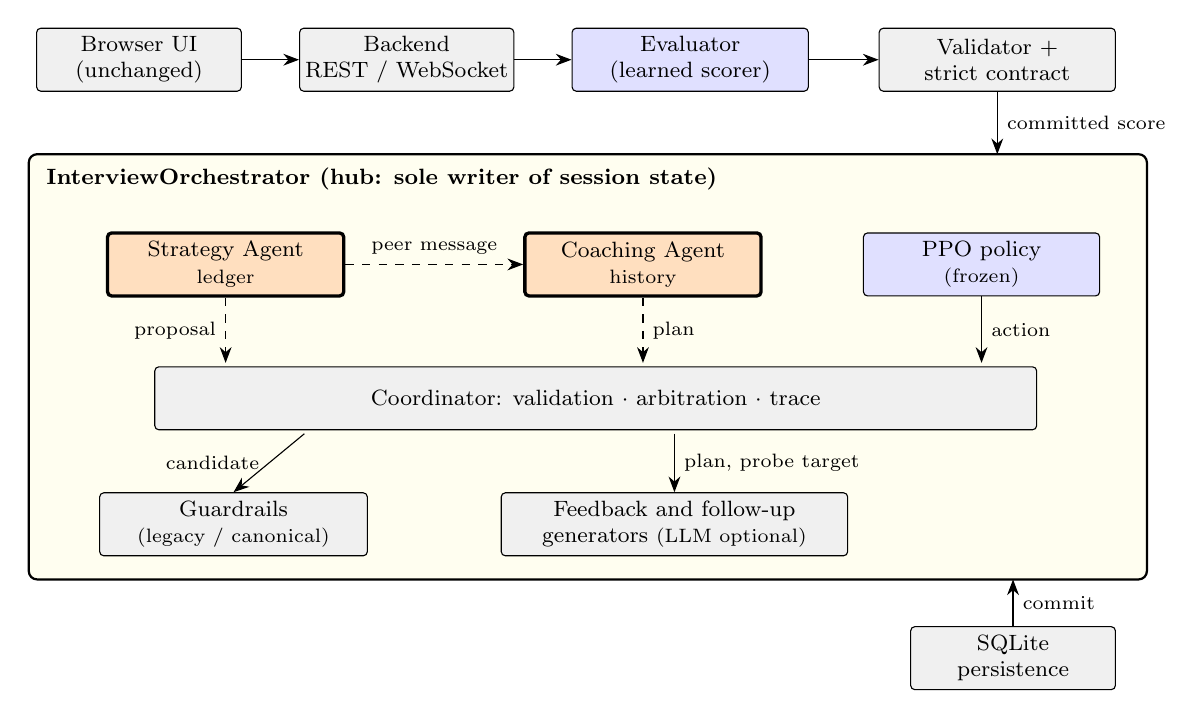
\begin{tikzpicture}[font=\footnotesize,
  box/.style={draw, rounded corners=1.5pt, minimum height=8mm, align=center, inner sep=2pt},
  det/.style={box, fill=gray!12},
  lrn/.style={box, fill=blue!12},
  agt/.style={box, fill=orange!25, very thick},
  arr/.style={-{Stealth[length=2mm]}, thin},
  darr/.style={-{Stealth[length=2mm]}, thin, dashed}]
% outside the hub
\node[det, minimum width=26mm] (ui) at (0.5,6.2) {Browser UI\\(unchanged)};
\node[det, minimum width=26mm] (be) at (3.9,6.2) {Backend\\REST / WebSocket};
\node[lrn, minimum width=30mm] (ev) at (7.5,6.2) {Evaluator\\(learned scorer)};
\node[det, minimum width=30mm] (val) at (11.4,6.2) {Validator +\\strict contract};
\draw[arr] (ui) -- (be); \draw[arr] (be) -- (ev); \draw[arr] (ev) -- (val);
% hub
\draw[rounded corners=3pt, thick, fill=yellow!6] (-0.9,-0.4) rectangle (13.3,5.0);
\node[anchor=north west, font=\footnotesize\bfseries] at (-0.8,4.95) {InterviewOrchestrator (hub: sole writer of session state)};
\node[agt, minimum width=30mm] (st) at (1.6,3.6) {Strategy Agent\\{\scriptsize ledger}};
\node[agt, minimum width=30mm] (co) at (6.9,3.6) {Coaching Agent\\{\scriptsize history}};
\node[lrn, minimum width=30mm] (pp) at (11.2,3.6) {PPO policy\\{\scriptsize (frozen)}};
\node[det, minimum width=112mm] (cd) at (6.3,1.9) {Coordinator: validation $\cdot$ arbitration $\cdot$ trace};
\node[det, minimum width=34mm] (gr) at (1.7,0.3) {Guardrails\\{\scriptsize (legacy / canonical)}};
\node[det, minimum width=44mm] (fb) at (7.3,0.3) {Feedback and follow-up\\generators {\scriptsize (LLM optional)}};
\node[det, minimum width=26mm] (db) at (11.6,-1.4) {SQLite\\persistence};
\draw[arr] (val.south) -- node[right]{\scriptsize committed score} (11.4,5.0);
\draw[darr] (st) -- node[above]{\scriptsize peer message} (co);
\draw[darr] (st.south) -- node[left]{\scriptsize proposal} (1.6,2.35);
\draw[darr] (co.south) -- node[right]{\scriptsize plan} (6.9,2.35);
\draw[arr] (pp.south) -- node[right]{\scriptsize action} (11.2,2.35);
\draw[arr] (2.6,1.45) -- node[left]{\scriptsize candidate} (gr.north);
\draw[arr] (7.3,1.45) -- node[right]{\scriptsize plan, probe target} (fb.north);
\draw[arr] (db.north) -- node[right]{\scriptsize commit} (11.6,-0.4);
\end{tikzpicture}
}
\caption{Implemented architecture. Shaded orange: the two added agents; blue: learned components; grey: deterministic infrastructure. Dashed arrows are typed proposals; agents never write state.}\label{fig:arch}
\end{figure}

\section{Orchestration, Arbitration and Validation}\label{sec:arbitration}
\begin{figure}[tbp]
\centering
\resizebox{0.97\textwidth}{!}{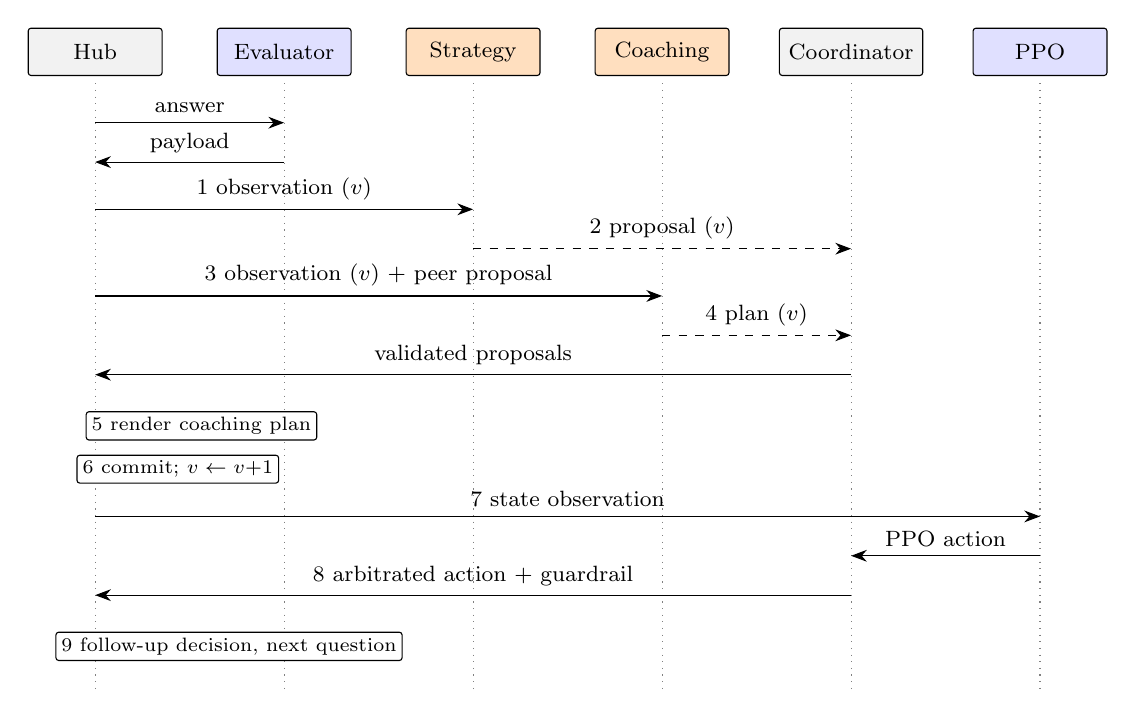
\begin{tikzpicture}[font=\footnotesize, x=1cm, y=1cm,
  life/.style={draw, rounded corners=1pt, minimum width=17mm, minimum height=6mm, align=center, fill=gray!10},
  msg/.style={-{Stealth[length=2mm]}, thin},
  dmsg/.style={-{Stealth[length=2mm]}, thin, dashed},
  note/.style={draw, fill=white, rounded corners=1pt, inner sep=2pt, font=\scriptsize}]
\def\xh{0} \def\xe{2.4} \def\xs{4.8} \def\xc{7.2} \def\xd{9.6} \def\xp{12}
\node[life] (hub) at (\xh,0) {Hub};
\node[life, fill=blue!12] (ev) at (\xe,0) {Evaluator};
\node[life, fill=orange!25] (st) at (\xs,0) {Strategy};
\node[life, fill=orange!25] (co) at (\xc,0) {Coaching};
\node[life] (cd) at (\xd,0) {Coordinator};
\node[life, fill=blue!12] (pp) at (\xp,0) {PPO};
\foreach \x in {\xh,\xe,\xs,\xc,\xd,\xp} \draw[gray, dotted] (\x,-0.4) -- (\x,-8.1);
\draw[msg] (\xh,-0.9) -- node[above]{answer} (\xe,-0.9);
\draw[msg] (\xe,-1.4) -- node[above]{payload} (\xh,-1.4);
\draw[msg] (\xh,-2.0) -- node[above]{1 observation $(v)$} (\xs,-2.0);
\draw[dmsg] (\xs,-2.5) -- node[above]{2 proposal $(v)$} (\xd,-2.5);
\draw[msg] (\xh,-3.1) -- node[above]{3 observation $(v)$ + peer proposal} (\xc,-3.1);
\draw[dmsg] (\xc,-3.6) -- node[above]{4 plan $(v)$} (\xd,-3.6);
\draw[msg] (\xd,-4.1) -- node[above]{validated proposals} (\xh,-4.1);
\node[note] at (\xh+1.35,-4.75) {5 render coaching plan};
\node[note] at (\xh+1.05,-5.3) {6 commit; $v \leftarrow v{+}1$};
\draw[msg] (\xh,-5.9) -- node[above]{7 state observation} (\xp,-5.9);
\draw[msg] (\xp,-6.4) -- node[above]{PPO action} (\xd,-6.4);
\draw[msg] (\xd,-6.9) -- node[above]{8 arbitrated action + guardrail} (\xh,-6.9);
\node[note] at (\xh+1.7,-7.55) {9 follow-up decision, next question};
\end{tikzpicture}
}
\caption{One interview turn as implemented (verbal path). Steps 1--4 happen before the hub commits; arbitration (8) follows the PPO suggestion. On the code-submission path only the Strategy proposal is collected.}\label{fig:flow}
\end{figure}
Figure~\ref{fig:flow} shows one turn. \textbf{Difficulty precedence} (deterministic code, evaluated by ablation rather than assumed optimal): (1) hard constraints (infrastructure failure forces Same; levels stay in $[1,5]$); (2) the guardrail layer, applied last to whichever candidate was selected, wins whenever a rule fires (G3 and G6 hold or raise difficulty, so this layer is not only a safety brake); (3) a validated Strategy proposal with confidence $\ge\tau$ and cited evidence supersedes the PPO action, recorded as a \emph{conflict}; (4) the PPO action, or the labelled non-RL heuristic when PPO is unavailable. A proposal that cannot take effect at the bounds is recorded as \emph{modified}. \textbf{Probe precedence:} the hard cap of two consecutive follow-ups, then a Strategy probe whose concept appeared in the evaluator's evidence earlier in this session and whose confidence is $\ge\tau$ (it may add a probe the thresholds would not trigger, or retarget the default one), then the hub's original threshold rule. The retargeted concept is passed to the template follow-up generator; the LLM prompt is not changed.

\textbf{PPO integration.} PPO keeps its role and its 6-D state and 3-action definitions; the checkpoint is frozen. Its action is one input to arbitration. The agents never see the PPO action before they propose, and the paper makes no claim that the agents improve PPO. Calling this multi-agent RL would be wrong: one policy is learned, and the agents are not trained.

\textbf{Guardrails.} The deployed hub uses an inline copy of the rule layer that differs from the module used by the training environment and the earlier policy study. A configuration key selects \texttt{legacy\_inline} (default; deployed behaviour) or \texttt{canonical}; both are reported separately. On a synthetic grid (39,930 points, $\mathit{hes}=1-\mathit{conf}$) the two disagree on 4,728 points (11.8\%) in G2, G6 and the no-override case; this is a property of the grid, not a deployment frequency, and a regression test pins it.

\begin{figure}[tbp]
\centering
\resizebox{\textwidth}{!}{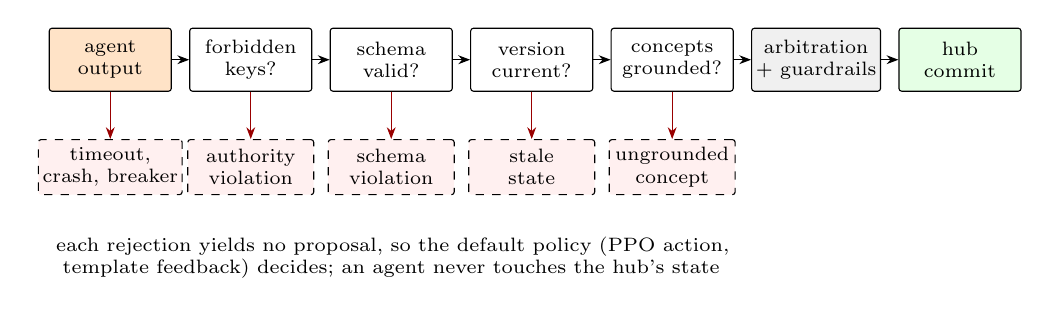
\begin{tikzpicture}[font=\scriptsize, node distance=2.2mm,
  s/.style={draw, rounded corners=1pt, minimum height=8mm, minimum width=15.5mm, align=center, inner sep=1.5pt},
  r/.style={draw, dashed, rounded corners=1pt, minimum height=7mm, minimum width=16mm, align=center, fill=red!6, inner sep=1.5pt},
  arr/.style={-{Stealth[length=1.5mm]}, thin}]
\node[s, fill=orange!22] (raw) {agent\\output};
\node[s, right=of raw] (au) {forbidden\\keys?};
\node[s, right=of au] (sc) {schema\\valid?};
\node[s, right=of sc] (sv) {version\\current?};
\node[s, right=of sv] (gr) {concepts\\grounded?};
\node[s, right=of gr, fill=gray!12] (ar) {arbitration\\+ guardrails};
\node[s, right=of ar, fill=green!10] (cm) {hub\\commit};
\foreach \a/\b in {raw/au,au/sc,sc/sv,sv/gr,gr/ar,ar/cm} \draw[arr] (\a) -- (\b);
\node[r, below=6mm of raw] (f0) {timeout,\\crash, breaker};
\node[r, below=6mm of au] (f1) {authority\\violation};
\node[r, below=6mm of sc] (f2) {schema\\violation};
\node[r, below=6mm of sv] (f3) {stale\\state};
\node[r, below=6mm of gr] (f4) {ungrounded\\concept};
\foreach \a/\b in {raw/f0,au/f1,sc/f2,sv/f3,gr/f4} \draw[arr, red!60!black] (\a) -- (\b);
\node[below=4mm of f2, text width=9cm, align=center] {each rejection yields no proposal, so the default policy (PPO action, template feedback) decides; an agent never touches the hub's state};
\end{tikzpicture}
}
\caption{Validation pipeline every proposal passes before arbitration. Each rejection yields no proposal; the default policy decides.}\label{fig:valid}
\end{figure}
\begin{table}[tbp]
\centering\footnotesize
\caption{Fault $\rightarrow$ detection $\rightarrow$ response for the agent layer, with the main limitation. In every case the state effect is none: agents cannot write state.}\label{tab:faults}
\begin{tabular}{>{\raggedright\arraybackslash}p{1.9cm}>{\raggedright\arraybackslash}p{2.7cm}>{\raggedright\arraybackslash}p{2.5cm}>{\raggedright\arraybackslash}p{4.3cm}}
\toprule
Fault & Detection & Response & Limitation\\
\midrule
crash & exception in call & no proposal; breaker failure & a deterministic crash opens the per-agent breaker for the rest of the session (cooldown 60\,s)\\
timeout & \texttt{wait\_for} & dropped; breaker failure & the worker thread cannot be killed; its late result is discarded\\
malformed / NaN & schema, NaN rejected & dropped & none beyond the schema\\
forbidden key & scan at any depth for 18 forbidden state and score keys & dropped (\emph{authority\_violation}) & finite list; schema rejection would also catch it (Sect.~\ref{sec:results})\\
stale / duplicate & version, turn, session; per (agent, version) & dropped & versions count commits only; the hub never retries, so duplicates arise only by injection\\
low confidence / no evidence & arbitration & rejected; PPO stands & $\tau$ is a heuristic\\
valid but harmful & guardrail layer last; bounds; step $\le1$ & modified or overridden & harm inside the region guardrails permit is accepted\\
ungrounded plan & concept $\notin$ evidence & plan dropped & string set membership; does not check text faithfulness\\
\bottomrule
\end{tabular}
\end{table}
Each agent has its own circuit breaker (threshold 2 failures, cooldown 60\,s), created per session, so sessions and agents are isolated; the LLM-service breaker is a separate, process-wide instance because that dependency is shared. Table~\ref{tab:faults} lists fault, detection, response and limitation.

\section{Experimental Methodology}\label{sec:method}
\paragraph{Evidence classes.} Every result is labelled. \textbf{REPLAY}: 64 recorded outputs of the production evaluator for 8 constructed technical questions with 8 constructed answers each (the evaluator itself is not executed), driven through the real hub; the replay candidate never improves, and follow-up questions are answered with the answer to their root question. \textbf{FAULT-INJECTED}: constructed faults in agent output. \textbf{SOCKET}: a local HTTP server with real timeouts. \textbf{SYNTHETIC}: authored feedback texts. No LLM weights were available, so the LLM service is stubbed as unavailable and the hub's non-LLM fallbacks serve follow-ups and feedback; the frozen PPO checkpoint runs unless a condition disables it. There is no human or live-model evidence in this paper.

\paragraph{Protocol and reproducibility.} The protocol, configuration, runners and analysis scripts were committed and tagged before any reported run; the protocol states metrics, units, predictions with criteria, deviations (three definitional fixes made after smoke runs and disclosed there) and exact commands. Each run records the commit, configuration hash and condition flags; results files are write-once, and tables are generated from them. The tag is local and carries no external timestamp.

\paragraph{XA: comparison and ablations.} Units are sessions: 8 recorded-answer sessions $\times$ 20 seeded question orders = 160 per condition, identical inputs across conditions, conditions interleaved in seeded random order. The 160 sessions reuse the same 64 answers and are therefore dependent; intervals are descriptive. Conditions: the original workflow (B0), without PPO (B7), with canonical guardrails (B0c); the full multi-agent configuration (M1); without the Strategy Agent (M2), the Coaching Agent (M3), arbitration (M4), the grounding check (M5), Strategy$\rightarrow$Coaching communication (M6), authority enforcement (M8); M1 without PPO (M7); M1 with canonical guardrails (M1c). Metrics: completion; \emph{authority} (every committed score equals the recorded evaluator score); \emph{transition validity} (levels in $[1,5]$, RL-phase steps $\le1$); level changes and reversals; agreement with the PPO action; guardrail firings; \emph{guardrail bypass} (final actions the guardrail layer would still override); conflicts; agent calls and valid-proposal rate; per-turn latency (pooled p50/p95). Level changes and reversals describe stability and are \emph{not} a quality measure.

\paragraph{XB: agent faults and ablated safeguards.} 8 sessions $\times$ 5 orders = 40 sessions per cell. Faults are injected in the agents' output at rate 0.3 per call (crash, timeout, malformed, forbidden key, stale version, NaN confidence) or on every call (a valid proposal that opposes the evidence; an ungrounded coaching plan), with the real agent running on all other calls. Variants: all safeguards, and each of authority enforcement, arbitration and grounding removed. A fault is \emph{contained} only if the session completes, committed scores remain authoritative and transitions are valid. Proportions use Clopper--Pearson exact intervals~\cite{cp34}.

\paragraph{XC: threshold decomposition and sensitivity (added after XA and XB).} XA's ``no arbitration'' condition (M4) removes four things at once: the confidence threshold $\tau$, the evidence requirement, the one-step bound and the guardrail layer, so it cannot show which one causes its behaviour. After seeing XA and XB we therefore registered a new experiment (a new protocol and tag, written and committed before any XC run, but designed after seeing XA and XB: it is a prospectively tagged experiment, not a preregistration made before the earlier results were known) that changes \emph{only} $\tau\in\{0,0.5,0.6,0.7,0.8,0.9\}$ on the same 160 replay sessions with every other check in force, and five predictions (C1--C5, Sect.~\ref{sec:results}). XC is a new experiment, not an amendment of XA or XB.

\paragraph{Statistics.} The registered XA and XB paired differences use a percentile bootstrap over sessions (10{,}000 resamples, fixed seed); latency differences use pooled-turn quantiles with sessions as resampling clusters. Because the 160 sessions per condition come from only 8 recorded answer sets, session-level intervals treat dependent units as independent and are too narrow~\cite{fw07}. We therefore add, labelled post hoc, a cluster bootstrap over the 8 recorded-answer sessions for the headline XA contrasts, and use it as the primary interval in XC. We call a difference an improvement only if the analysis supports it, and none of XA's behavioural metrics can support that claim.

\paragraph{Pre-registered predictions.} XA: A1--A3 (completion, authority and transition validity everywhere), A4 (no Strategy Agent reproduces the original trajectory), A5 (ablating coaching, communication, grounding or authority leaves difficulty paths unchanged without faults), A6 (no arbitration $\Rightarrow$ guardrail bypass; full $\Rightarrow$ none), A7 (the agents change the difficulty path in $\ge50\%$ of sessions), A8 (median latency overhead $<50$\,ms), A9 (with PPO unavailable the agents still change the path in $\ge50\%$ of sessions), A10 (canonical guardrails change at least one path). XB: B1--B6 (Sect.~\ref{sec:results}). The outcome of every prediction is reported, including contradictions.

\section{Results}\label{sec:results}
All results are REPLAY or FAULT-INJECTED unless stated; no LLM ran. Sessions within a condition are dependent (Sect.~\ref{sec:method}).

\subsection{Coordination and ablations (XA, RQ1, RQ3)}
\begin{table}[tbp]
\centering\scriptsize\setlength{\tabcolsep}{3pt}
\caption{XA, 160 replay sessions per condition (mean per session unless counts). compl./auth./trans.: numbers of the 160 sessions that completed, kept committed scores authoritative, kept valid transitions. chg./rev.: level changes and reversals; agr.: share of RL-phase decisions equal to the PPO (or heuristic) action; gfire: guardrail firings; strat.: decisions whose final source is the Strategy Agent; byp.: sessions with a guardrail bypass; p50/p95: pooled per-turn latency in ms; calls: agent calls.}\label{tab:xa}
\resizebox{\textwidth}{!}{\begin{tabular}{lcccrrrrrrrrr}
\toprule
Cond. & compl. & auth. & trans. & chg. & rev. & agr. & gfire & strat. & byp. & p50 & p95 & calls\\
\midrule
B0 & 160 & 160 & 160 & 15.119 & 11.744 & 0.626 & 9.588 & 0.0 & 0 & 0.546 & 2.056 & -- \\
B7 & 160 & 160 & 160 & 2.675 & 1.256 & -- & 3.831 & 0.0 & 0 & 0.463 & 1.059 & -- \\
B0c & 160 & 160 & 160 & 15.119 & 11.744 & 0.626 & 9.588 & 0.0 & 0 & 0.553 & 2.004 & -- \\
M1 & 160 & 160 & 160 & 12.45 & 9.869 & 0.4 & 6.838 & 6.669 & 0 & 1.589 & 4.411 & 47.68 \\
M2 & 160 & 160 & 160 & 15.119 & 11.744 & 0.626 & 9.588 & 0.0 & 0 & 1.218 & 3.513 & 23.25 \\
M3 & 160 & 160 & 160 & 12.45 & 9.869 & 0.4 & 6.838 & 6.669 & 0 & 1.118 & 3.189 & 23.84 \\
M4 & 160 & 160 & 160 & 2.225 & 1.0 & 0.014 & 0.0 & 19.619 & 3 & 1.573 & 4.357 & 47.68 \\
M5 & 160 & 160 & 160 & 12.45 & 9.869 & 0.4 & 6.838 & 6.669 & 0 & 1.581 & 4.553 & 47.68 \\
M6 & 160 & 160 & 160 & 12.45 & 9.869 & 0.4 & 6.838 & 6.669 & 0 & 1.592 & 4.46 & 47.68 \\
M8 & 160 & 160 & 160 & 12.45 & 9.869 & 0.4 & 6.838 & 6.669 & 0 & 1.575 & 4.35 & 47.68 \\
M7 & 160 & 160 & 160 & 2.706 & 1.312 & -- & 3.812 & 9.037 & 0 & 1.502 & 2.968 & 47.68 \\
M1c & 160 & 160 & 160 & 12.45 & 9.869 & 0.4 & 6.838 & 6.669 & 0 & 1.573 & 4.534 & 47.68 \\
\bottomrule
\end{tabular}
}
\end{table}
\begin{table}[tbp]
\centering\scriptsize\setlength{\tabcolsep}{3pt}
\caption{XA paired differences (A$-$B) over the same 160 sessions: share of sessions with a different difficulty path, paired mean differences with 95\% percentile-bootstrap intervals, and the pooled-turn median latency difference. Intervals are descriptive (dependent sessions).}\label{tab:xapaired}
\resizebox{\textwidth}{!}{\begin{tabular}{lrcccc}
\toprule
A$-$B & path$\ne$ & $\Delta$ level chg. & $\Delta$ reversals & $\Delta$ PPO agree & $\Delta$ p50 ms\\
\midrule
M1$-$B0 & 1.0 & $-$2.669 [$-$3.188,$-$2.131] & $-$1.875 [$-$2.275,$-$1.462] & $-$0.226 [$-$0.244,$-$0.208] & +1.043 [+1.000,+1.079] \\
M2$-$B0 & 0.0 & 0 & 0 & 0 & +0.672 [+0.646,+0.698] \\
M3$-$M1 & 0.0 & 0 & 0 & 0 & $-$0.471 [$-$0.511,$-$0.425] \\
M4$-$M1 & 1.0 & $-$10.225 [$-$10.544,$-$9.900] & $-$8.869 [$-$9.275,$-$8.463] & $-$0.387 [$-$0.403,$-$0.370] & $-$0.016 [$-$0.065,+0.033] \\
M5$-$M1 & 0.0 & 0 & 0 & 0 & $-$0.008 [$-$0.059,+0.037] \\
M6$-$M1 & 0.0 & 0 & 0 & 0 & +0.004 [$-$0.030,+0.053] \\
M8$-$M1 & 0.0 & 0 & 0 & 0 & $-$0.013 [$-$0.057,+0.032] \\
M7$-$B7 & 0.025 & +0.031 [+0.000,+0.081] & +0.056 [+0.006,+0.125] &  & +1.039 [+0.996,+1.070] \\
B0c$-$B0 & 0.0 & 0 & 0 & 0 & +0.008 [$-$0.019,+0.027] \\
M1c$-$M1 & 0.0 & 0 & 0 & 0 & $-$0.016 [$-$0.055,+0.032] \\
\bottomrule
\end{tabular}
}
\end{table}
Every condition completed all 160 sessions, kept every committed score equal to the recorded evaluator output, and kept every level in $[1,5]$ with RL-phase steps of at most one (A1--A3; exact 95\% lower bound for 160/160: 0.977~\cite{cp34}). Removing the Strategy Agent reproduced the original workflow's difficulty, score and question paths in every session (A4), and removing coaching, communication, grounding or authority enforcement reproduced the full configuration's paths (A5): without faults these components do not influence difficulty or probes, as designed.

With both agents the difficulty path differed from the original in all 160 sessions (A7). Level changes fell from 15.12 to 12.45 per session ($-2.67$, interval $[-3.19,-2.13]$) and reversals from 11.74 to 9.87 ($-1.88$, $[-2.28,-1.46]$); agreement with the PPO action fell from 0.626 to 0.400; sessions contained on average 0.59 more turns ($[+0.34,+0.85]$) because proactive probes added follow-ups. In 11.9 decisions per session a Strategy proposal superseded the PPO action before the guardrail layer. The session-level intervals above treat the 160 dependent sessions as independent. A post hoc cluster bootstrap over the 8 recorded-answer sessions gives wider intervals: level changes \phchgmean{} \phchgci{}, reversals \phrevmean{} \phrevci{}, agreement with the PPO action \phagrmean{} \phagrci{} (all 8 clusters share the sign), and extra turns \phfumean{} \phfuci{}, where only \phfusame{} of the 8 recorded sessions shows an increase, so the extra-turn effect is driven by a single recorded session and should not be generalised. In a post hoc leave-one-cluster-out analysis the level-change interval excludes zero when the opposing set is dropped ($-3.76$, $[-4.81,-2.78]$) but includes zero when any one of the other seven is dropped, so the sign is better supported than the interval; the agreement decrease excludes zero in all eight drops. Level changes and reversals decreased in 7 of the 8 answer sets; the exception is the set behind all extra turns. Across the 160 sessions the Strategy Agent emitted \scTotal{} proposals: \scRemEight{} \emph{remediate} (confidence 0.80), \scRecEight{} and \scRecSeven{} \emph{recover} (0.80 and 0.70) and \scSteady{} \emph{steady} (0.45); it never emitted a \emph{stretch} proposal (\scStretch{}), so in these experiments it only held or lowered difficulty and the stretch rule is unexercised. These are stability and coordination measures; fewer reversals are not evidence of better interviewing, and the replay candidate cannot reveal whether the agents' proposals were pedagogically appropriate.

Two results were not anticipated. (i) \emph{Arbitration is not only a precedence rule.} Without it (M4), steady proposals of confidence 0.45 replaced the PPO action almost everywhere: level changes fell to 2.2 per session, agreement with PPO to 0.014, guardrails never fired, and 3 sessions contained a final action the guardrail layer would still override; M4 removes four checks at once, so this does not by itself identify the threshold; XC (below) isolates it. (ii) With PPO unavailable the agents changed the difficulty path in only 4 of 160 sessions (2.5\%; A9 contradicted): on this replay the Strategy Agent mostly agrees with the labelled non-RL heuristic. Canonical guardrails changed no path (A10 contradicted): replay has no audio, so confidence and hesitation stay at their defaults and the divergent regions of the two implementations (G2, G6) are never reached; the 11.8\% grid disagreement says nothing about their frequency in use.

\emph{Cost.} Pooled per-turn latency rose from \xaBzeroMed{} to \xaMoneMed{}\,ms at the median and from \xaBzeroHigh{} to \xaMoneHigh{}\,ms at the 95th percentile (median difference $+1.04$\,ms, $[+1.00,+1.08]$), 47.7 agent calls per session. The agents are in-process rules, so there are no model calls and no token counts; an LLM-backed agent would add its own latency, which we did not measure.

\begin{table}[tbp]
\centering\scriptsize\setlength{\tabcolsep}{3pt}
\caption{Registered predictions and outcomes. XA (above) and XB (below).}\label{tab:preds}
\begin{tabular}{lp{7.6cm}l}
\toprule
ID & Prediction & Outcome\\
\midrule
A1 & completion 100\% in every condition & Supported \\
A2 & committed scores equal the recorded evaluator output in every session of every condition & Supported \\
A3 & difficulty levels stay within [1,5], and every RL-phase decision moves by at most one level, in every session of every condition & Supported \\
A4 & M2 (no Strategy Agent) reproduces B0 (difficulty, score and question paths) in every session & Supported \\
A5 & M3, M5, M6, M8 reproduce M1's difficulty/score/question paths in every session (fault-free) & Supported \\
A6 & M4 (no arbitration) has guardrail\_bypass>0 in >=1 session; M1 has 0 in all & Supported \\
A7 & M1 differs from B0 in difficulty path in >=50\% of sessions & Supported \\
A8 & median per-turn latency M1 - B0 < 50 ms (pooled turns) & Supported \\
A9 & with PPO unavailable, M7 differs from B7 in difficulty path in >=50\% of sessions & Contradicted \\
A10 & canonical guardrails change the difficulty path in >=1 session vs legacy (B0c vs B0) & Contradicted \\
\bottomrule
\end{tabular}
\\[2mm]
\begin{tabular}{lp{7.6cm}l}
\toprule
ID & Prediction & Outcome\\
\midrule
B1 & variant=full: every fault cell completes, keeps committed scores authoritative and transitions valid; no guardrail bypass, no ungrounded leak & Supported \\
B2 & forbidden\_key: full -> authority\_violation>0 and schema\_violation==0; no\_authority -> authority\_violation==0, schema\_violation>0; containment 100\% in both & Supported \\
B3 & adversarial\_valid: no\_arbitration has guardrail\_bypass>0 in >=1 session; full has 0 & Supported \\
B4 & ungrounded coaching: no\_grounding leaks (>=1 session); full has 0 leaks and rejects plans & Supported \\
B5 & strategy timeout (full): pooled p95 per-turn latency exceeds the clean M1 p95 by >=100 ms & Supported \\
B6 & at fault rate 0.3, >=80\% of sessions see the per-agent breaker open at least once (crash/malformed/stale/nan cells) & Contradicted \\
\bottomrule
\end{tabular}

\end{table}

\subsection{Agent faults and safeguards (XB, RQ2)}
\begin{table}[tbp]
\centering\scriptsize\setlength{\tabcolsep}{3pt}
\caption{XB, 40 sessions per fault and variant (160 per fault over four variants). inj.: injected faulty or harmful outputs in the full variant; compl./auth./trans.: sessions completed, with authoritative scores, with valid transitions; bypass: sessions with a guardrail-overridable final action (full / arbitration removed); leak: sessions in which an ungrounded concept was emphasised (full / grounding removed); brk.: sessions in which the per-agent breaker opened (full); p95: pooled per-turn latency.}\label{tab:xb}
\resizebox{\textwidth}{!}{\begin{tabular}{lrcccccrr}
\toprule
Fault & inj. & compl. & auth. & trans. & bypass & leak & brk. & p95\\
 & (full) & \multicolumn{3}{c}{all 4 variants} & full/no-arb. & full/no-gr. & full & ms\\
\midrule
coach:crash & 154 & 160/160 & 160/160 & 160/160 & 0 / 1 & 0 / 0 & 29 & 4.09 \\
coach:malformed & 154 & 160/160 & 160/160 & 160/160 & 0 / 1 & 0 / 0 & 29 & 4.85 \\
coach:stale & 154 & 160/160 & 160/160 & 160/160 & 0 / 1 & 0 / 0 & 29 & 4.33 \\
coach:ungrounded & 950 & 160/160 & 160/160 & 160/160 & 0 / 1 & 0 / 40 & 0 & 4.45 \\
strat:adversarial\_valid & 930 & 160/160 & 160/160 & 160/160 & 0 / 38 & 0 / 0 & 0 & 4.5 \\
strat:crash & 152 & 160/160 & 160/160 & 160/160 & 0 / 34 & 0 / 0 & 29 & 3.83 \\
strat:forbidden\_key & 152 & 160/160 & 160/160 & 160/160 & 0 / 34 & 0 / 0 & 29 & 3.86 \\
strat:malformed & 152 & 160/160 & 160/160 & 160/160 & 0 / 34 & 0 / 0 & 29 & 3.62 \\
strat:nan\_confidence & 152 & 160/160 & 160/160 & 160/160 & 0 / 34 & 0 / 0 & 29 & 4.14 \\
strat:stale & 152 & 160/160 & 160/160 & 160/160 & 0 / 34 & 0 / 0 & 29 & 4.04 \\
strat:timeout & 152 & 160/160 & 160/160 & 160/160 & 0 / 34 & 0 / 0 & 29 & 154.38 \\
\bottomrule
\end{tabular}
}
\end{table}
\textbf{Containment is at ceiling and does not discriminate the safeguards.} In every fault cell and variant all sessions completed with authoritative scores and valid transitions (B1; Table~\ref{tab:xb}); the hub's own bounds and authoritative scoring already enforce these properties, so the safeguards matter for other properties. \textbf{Authority check.} For a forbidden key (152 injections) the full configuration classified all as authority violations and none as schema violations; with enforcement removed all 152 became schema violations and containment was unchanged (B2): the strict schema alone contains such output, and the authority check is classification and defence in depth. \textbf{Arbitration.} A valid proposal opposing the evidence (930 injections) produced final actions the guardrails would override in 38 of 40 sessions without arbitration and in none with it (B3); without arbitration the guardrail layer is skipped entirely, so the same bypass appeared in 34 of 40 sessions of the Strategy fault cells where proposals were dropped or steady. In the full configuration the adversarial proposal was nevertheless the final source of 10.8 decisions per session on average (a guardrail may override it afterwards): a well-formed, confident, evidenced proposal that is wrong cannot be detected by these checks, only bounded by the guardrails and the one-step limit. \textbf{Grounding.} All 950 ungrounded plans were rejected in the full configuration; without the check an ungrounded concept was emphasised in 40 of 40 sessions (B4). \textbf{Timeouts.} A timing-out Strategy Agent raised the pooled p95 per-turn latency from 4.4 to 154.4\,ms, about the configured 150\,ms timeout (B5). \textbf{Breaker.} With a fault rate of 0.3 the per-agent breaker opened in 29 of 40 sessions (72.5\%; the same count in every fault type, because all share one seeded fault schedule per session) and, with a 60\,s cooldown longer than a session, silenced the agent for the rest of that session; the registered threshold of 80\% was not met (B6 contradicted), and the cost of the breaker design is lost agent availability after one burst.

\subsection{Threshold decomposition and sensitivity (XC)}
\begin{table}[tbp]
\centering\scriptsize\setlength{\tabcolsep}{3pt}
\caption{XC (REPLAY, 160 sessions per row, mean per session): only $\tau$ changes; evidence requirement, one-step bound and guardrails stay in force. chg./rev.: level changes and reversals; agr.: share of RL-phase decisions equal to the PPO action; strat.: decisions whose final source is the Strategy Agent; gfire: guardrail firings; byp.: sessions with a guardrail bypass. Cluster-bootstrap intervals over the 8 recorded-answer sessions are in the released summary file.}\label{tab:xc}
\begin{tabular}{rcccccc}\toprule
$\tau$ & chg. & rev. & agr. & strat. & gfire & byp.\\
\midrule
0.0 & 2.225 & 1.000 & 0.014 & 16.075 & 3.544 & 0 \\
0.5 & 12.450 & 9.869 & 0.400 & 6.669 & 6.838 & 0 \\
0.6 & 12.450 & 9.869 & 0.400 & 6.669 & 6.838 & 0 \\
0.7 & 12.450 & 9.869 & 0.400 & 6.669 & 6.838 & 0 \\
0.8 & 12.450 & 9.819 & 0.404 & 6.594 & 6.863 & 0 \\
0.9 & 15.119 & 11.744 & 0.626 & 0.000 & 9.588 & 0 \\
\bottomrule
\end{tabular}

\end{table}
Setting $\tau=0$ alone reproduced M4's collapse (level changes \xctauzerochg{}, PPO agreement \xctauzeroagr{}, as in M4) with no guardrail bypass in any session (C1): ungated \emph{steady} proposals of confidence 0.45 replace the PPO action almost everywhere, and the guardrail layer then fires on a smaller share of decisions. The collapse is therefore caused by the missing confidence threshold and not by the removed guardrails, bound or evidence check; the bypass seen in M4 is a separate consequence of skipping the guardrail layer. The full configuration reproduced XA's M1 paths in every session at $\tau=0.6$ (C2, a determinism check) and $\tau=0.5$ gave identical paths (C3). Behaviour was flat for $0.5\le\tau\le0.8$ and the Strategy Agent was silent at $\tau=0.9$ (identical to the original workflow's agreement of 0.626; C4, C5): the realised confidences are only 0.45, 0.70 and 0.80 (Sect.~\ref{sec:results}, XA), so any $\tau$ in $(0.45,0.70]$ admits exactly the same proposals, $\tau=0.8$ excludes only the 0.70 \emph{recover} proposals and $\tau=0.9$ admits none; the formula separates \emph{steady} from evidenced proposals and hardly distinguishes among evidenced ones. All \xcsupported{} registered XC predictions were supported. This shows that the threshold matters; the plateau is a consequence of the two-valued confidence, not evidence that behaviour is robust to the threshold, and it does not show that 0.6 is better than another value for interviewing.

\subsection{Grounding probe, rebuilt (XD)}
\begin{table}[tbp]
\centering\scriptsize\setlength{\tabcolsep}{3pt}
\caption{XD: constructed feedback texts that disagree with their intended label, over applicable payloads, for the lexical validator, on three subsets of the 64 recorded evaluator payloads.}\label{tab:xd}
\begin{tabular}{lccc}
\toprule
Category & ALL (64) & NO\_OVERLAP (47) & RELABELLED (64)\\
\midrule
C0 faithful & 17/64 & 0/47 & 0/64 \\
C1 verbatim missing as correct & 0/57 & 0/40 & 0/57 \\
C2 verbatim incorrect as correct & 0/10 & 0/4 & 0/10 \\
C3 narrative correctly explained m & 0/57 & 0/40 & 0/57 \\
C4 truncated paraphrase credit & 40/57 & 40/40 & 57/57 \\
C5 score leak & 0/64 & 0/47 & 0/64 \\
C6 generic fluff & 0/64 & 0/47 & 0/64 \\
\bottomrule
\end{tabular}

\end{table}
All 64 stored payloads contain placeholder concept text, and \xdOverlap{} contain the same placeholder string in both the covered and the missing list. In the original accounting 17 of 64 faithful texts were rejected; on the 47 payloads without overlap and on all 64 with numbered placeholders, faithful texts were accepted in 47/47 and 64/64: the 17 rejections were an artefact of contradictory evidence, not validator behaviour. The correction goes the other way for credit claims: truncated paraphrases of unsupported credit were accepted in 40 of 57 applicable cases originally, but in 40/40 on the overlap-free subset and 57/57 with numbered placeholders (95\% interval for 57/57: [0.937,1.000]). The lexical check rejects verbatim claims, narrative restatements of missing concepts, score leaks and generic text in every applicable case, and accepts paraphrased unsupported credit in every applicable case. The evaluation is deterministic and constructed; it says nothing about LLM outputs.

\section{Corrections to an Earlier Audit (RQ4)}\label{sec:carry}
An earlier audit of this system's single-controller version (a mechanism-by-fault ablation, E1, over five registered fault classes) contained claims that did not survive review. We list each with the correction and its evidence; none of the earlier stored results was overwritten.
\paragraph{Prediction count.} The earlier manuscript reported that all 14 registered predictions held. The registered prediction for the no-guardrail variant (V2) was that invariant I7 (no difficulty increase after a score below 0.30) would be violated \emph{more often} than in the full system. Recomputing from the stored runs, I7 was violated in 3 of 8 sessions for V2 and 7 of 8 for the full system, so \textbf{13 of 14 predictions held and one was contradicted}; the earlier analysis had applied a weaker criterion (any violation).
\paragraph{Malformed scorer output.} The earlier text implied the shipped system committed malformed scores in production. At the hub seam with an injected evaluator (synthetic fault injection), a non-numeric, \texttt{None}, NaN, out-of-range or string score was committed after repair to 0.0 or a clamped value in every session of that cell. In the deployed backend wrapper, however, \texttt{None} and non-numeric scores already raise (so the hub fails closed), and only NaN (to 0.0) and out-of-range numbers (1.7 to 1.0, $-0.3$ to 0.0) are repaired; the evaluator itself clamps to $[0,1]$. A regression test pins this behaviour. The strict contract is therefore defence in depth at the hub seam, not the fix of a demonstrated production defect.
\paragraph{Historical reproducibility.} The strict contract is now default-on, so re-running E1 with defaults gives different results in the malformed-score cells. Under explicit historical flags (strict contract off, breaker disabled) a re-run of all \xeEoneRows{} sessions was byte-identical to the stored file (\xeEoneDiff{} sessions differing; SHA-256 equal). Experiments therefore carry an explicit configuration.
\paragraph{Guardrail divergence.} The deployed orchestrator uses an inline rule layer that differs from the module used by the training environment and the earlier policy study. An earlier figure of 12.4\% disagreement on a synthetic grid included an artefact of the comparison script (the canonical function reads difficulty values at most 1.0 as already normalised); with a normalised input the disagreement is 4,728 of 39,930 points (11.8\%; 7.4\% on a full grid). A configuration key selects either implementation and both are tested; the shipped default is unchanged.
\paragraph{Scorer semantics.} The evaluator's calibration assumes a sigmoid-bounded cross-encoder score. The pinned library range applies a sigmoid by default for a single-label head (verified in the source of version 2.7.0), but the installed 6.1.0 returns raw logits (values 1.55 and $-7.95$ for two test pairs, equal to the sigmoid-inverse of the explicit-activation outputs). The loader now passes the activation explicitly; a test checks the loader for both keyword conventions and, where weights are materialised, that scores are probabilities equal to the sigmoid of the logits.
\paragraph{Grounding artefact.} See Sect.~\ref{sec:results}: the 17 false rejections were artefacts, and the unsupported-credit acceptance is higher than reported.
\paragraph{Circuit breaker.} In the earlier breaker, any HTTP response counted as success. Against a service that answers every request with HTTP 503, the historical semantics sent \bfivezerothreeerrfivezerothreelegacy{} requests over a 24-turn replay session at a median \bfivezerothreemederrfivezerothreelegacy{}\,s per turn, whereas treating 5xx as failure sent \bfivezerothreeerrfivezerothreefixed{} requests at \bfivezerothreemederrfivezerothreefixed{}\,s per turn; the 24 committed scores were identical in all variants (SOCKET, one session). A cancelled half-open probe previously left the breaker rejecting all calls; it is now released.
\paragraph{Breaker timing re-run.} The breaker timings were re-measured with current code against a local socket server with real six-second timeouts (a new SOCKET run, not a reproduction; one 24-turn replay session). Per-turn medians in seconds, new (earlier): hanging service without the breaker \efivehangBnew{} (\efivehangBold{}); with the breaker at pacing $P{=}30$, 60 and 120\,s \efivehangSPthreezeronew{} (\efivehangSPthreezeroold{}), \efivehangSPsixzeronew{} (\efivehangSPsixzeroold{}) and \efivehangSPonetwozeronew{} (\efivehangSPonetwozeroold{}); healthy \efiveokSPsixzeronew{} (\efiveokSPsixzeroold{}), refusing \efiverefuseSPsixzeronew{} (\efiverefuseSPsixzeroold{}), recovery \efiverecoverSPsixzeronew{} (\efiverecoverSPsixzeroold{}). HTTP attempts were unchanged in the hanging scenarios (\efivehangBnewhttp{}, \efivehangSPthreezeronewhttp{}, \efivehangSPsixzeronewhttp{}). One run on one machine, so differences of a few hundredths of a second are not interpreted.

\section{Discussion}
\textbf{What the agents add.} Beyond the earlier hub, the contribution that can be defended is structural: two stateful agents take real decisions (difficulty proposals, probes, coaching plans) through typed messages, with an authority matrix enforced in code and arbitration that is transparent when the agents contribute nothing (identical trajectories with no usable agent). The Strategy Agent's ledger is what a threshold rule or PPO's 6-D state lacks; the replay shows that it changes the difficulty path in every session, but \emph{not} whether the change is better.

\textbf{What the safeguards do.} The ablations separate roles. Schema validation contains malformed and forbidden output; the authority check adds classification; the confidence threshold prevents ungated ``steady'' proposals from overriding PPO (isolated in XC; the removal of arbitration in XA changes four checks at once); guardrail precedence prevents bypass; grounding prevents ungrounded emphasis; the per-agent breaker bounds repeated failures at the cost of availability. None of these detects a well-formed, confident, wrong proposal, which was followed in a measurable share of decisions; only bounds and guardrails limit its effect.

\textbf{Why two agents rather than one rules engine?} The evidence does not show that two agents are needed. Removing the Coaching Agent changes no difficulty, score or question path (A5), so one merged component would have behaved identically on these metrics. The split is an authority and state boundary: each agent has its own private ledger, its own typed output and its own breaker, so a fault in one does not remove the other (XB), and coaching can be audited and disabled without touching difficulty. Whether this modularity is worth its overhead for a system this size, against a single rules engine with the same ledger, was not tested.

\textbf{Is it multi-agent?} By the weak notion of agency~\cite{wj95}, each agent has private persistent state, reacts to observations, makes pro-active proposals (a probe the thresholds would not trigger) and communicates (Strategy to Coaching through the coordinator). Their decision logic is rule-based; they are not LLM agents, do not negotiate, and the system remains centrally orchestrated. This is bounded-authority role specialisation, not decentralised intelligence, and PPO's role is unchanged.

\textbf{Relation to the tracks.} The work fits agent-native development and lifecycle engineering (typed contracts, authority, fault containment, regression-tested integration) better than core multi-agent collaboration; the authority matrix, containment of faulty agents and breaker behaviour also relate to the security-and-resilience track. We have not verified the official call text (Sect.~\ref{sec:limits}).

\section{Limitations and Threats to Validity}\label{sec:limits}
\textbf{No live model and no human evidence.} All data are replayed recorded evaluator payloads for 8 constructed questions and 64 constructed answers, injected faults, or one local socket server. The agents are rule-based; no LLM output was produced; follow-ups and feedback came from the hub's template fallbacks. We make no claim about coaching quality, learning, evaluator validity, or that the agents improve PPO. \textbf{Replay candidate.} Scores are fixed per answer and follow-ups reuse the root answer, so the effect of any decision on later answers cannot appear. \textbf{Dependent sessions.} The 160 XA sessions per condition reuse 64 answers; intervals are descriptive. \textbf{Metrics.} Level changes, reversals and agreement with PPO are behaviour measures, not quality measures. \textbf{Unexercised regions.} Replay has no audio, so confidence and hesitation are constant and the divergent guardrail regions are not exercised; the XA result that canonical and legacy guardrails give identical paths is specific to this input. \textbf{Post hoc additions.} XC was designed after XA and XB showed that M4 bundles four checks; its protocol and tag precede its runs, but its motivation depends on earlier results. The cluster-bootstrap intervals for XA are post hoc. With 8 recorded answer sets, even cluster intervals are coarse. \textbf{Registered but not pre-confirmed.} A9, A10 and B6 were contradicted; three metric definitions were fixed after smoke runs (disclosed in the protocol). \textbf{Agent design.} Thresholds ($\tau$, ledger parameters) were fixed in advance, not tuned, and are heuristics; the agents are not claimed to be optimal. Persistent memory is restored from a session snapshot, but a retried turn re-uses the first observation of that turn. \textbf{Coverage.} The coaching renderer is exercised on the verbal path only; the code-submission path collects only the Strategy proposal. The Strategy Agent never proposed a harder level in these experiments (no \emph{stretch} proposal), so that rule is untested here. \textbf{Trust boundary.} The agents are in-process trusted code: the authority matrix constrains what their outputs can do (schema, forbidden keys, version, arbitration), not what their code could do, so a malicious agent implementation is out of scope. \textbf{Deployment surface.} In the shipped backend the layer is enabled only by a server-side environment variable (default off; clients cannot set it), added after the main experiments (which used the constructor option). The web client has no display of agent output; the shipped-path server run used recorded evaluator payloads. After a restart the agents' ledgers, decision records and call counters are restored from the snapshot (breaker state is not). \textbf{Environment.} Runs used one Python environment outside the repository's dependency pins. The historical 407-test baseline was not reproduced as a whole: the 28 frontend tests pass, but the Python suite has 23 failures and 36 errors (Docker sandbox, model downloads, one documented known failure), the same 59 test identifiers as in a clean export of the frozen baseline commit, so a full green run was not obtained; at the audited head 421 Python tests pass (306 in the frozen export) with no new failure. \textbf{Provenance.} Protocol tags are local and carry no external timestamp; the reference list was checked through a search interface (titles, venues and abstracts) and full texts were not read; the official venue instructions could not be retrieved from the authors' environment.

\section{Conclusion}
We extended an existing orchestrated interview-practice workflow with two stateful, bounded-authority agents whose typed proposals pass a deterministic coordinator, arbitration and a hub that alone commits state, while the evaluator, PPO policy and workflow are preserved. On replayed recorded evaluator output the agents change difficulty paths in every session, the arbitration layer is transparent when no agent contributes, and agent faults are contained at the cost of a small per-turn latency; the ablations show which safeguard protects which property and that none detects a well-formed but wrong proposal. Re-running and correcting an earlier audit gave 13 of 14 predictions, a narrower malformed-score claim, an explicit and byte-reproducible historical configuration, and a larger grounding weakness than first reported. Whether the agents improve interviews, coaching or learning remains untested and needs a live model and human candidates.


\bibliographystyle{splncs04}
\bibliography{refs}
\end{document}
